\begin{figure}[t]\centering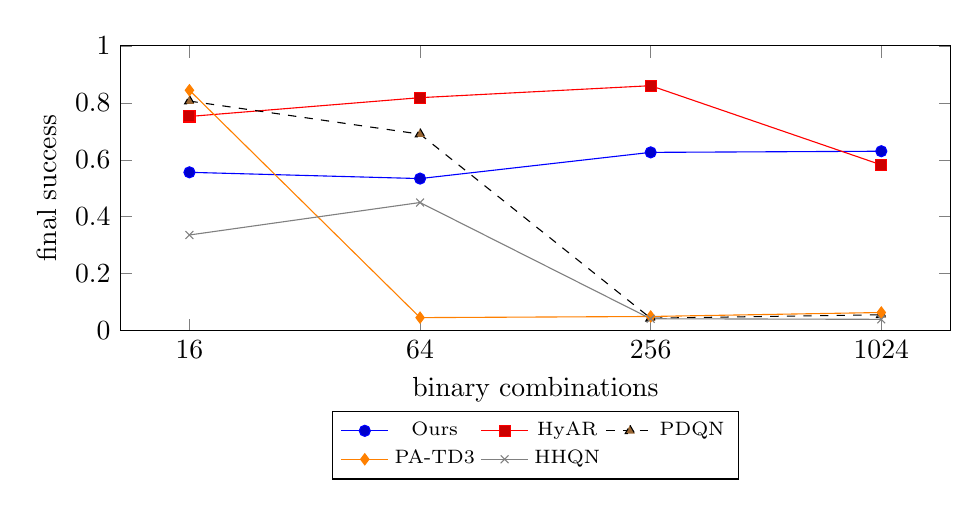
\begin{tikzpicture}\begin{axis}[width=\linewidth,height=5.2cm,ymin=0,ymax=1,xlabel={binary combinations},ylabel={final success},xtick={1,2,3,4},xticklabels={16,64,256,1024},legend style={font=\scriptsize,at={(.5,-.28)},anchor=north,legend columns=3}]
\addplot+[blue,mark=*] coordinates {(1,.556)(2,.534)(3,.626)(4,.630)};\addlegendentry{Ours}
\addplot+[red,mark=square*] coordinates {(1,.752)(2,.818)(3,.860)(4,.582)};\addlegendentry{HyAR}
\addplot+[black,dashed,mark=triangle*] coordinates {(1,.806)(2,.690)(3,.044)(4,.056)};\addlegendentry{PDQN}
\addplot+[orange,mark=diamond*] coordinates {(1,.844)(2,.046)(3,.050)(4,.064)};\addlegendentry{PA-TD3}
\addplot+[gray,mark=x] coordinates {(1,.336)(2,.450)(3,.042)(4,.040)};\addlegendentry{HHQN}
\end{axis}\end{tikzpicture}\caption{HardMove success versus joint binary combinations. Main panel shows major baselines; Appendix lists all values.}\label{fig:hmsuccess}\end{figure}
